\documentclass[border=10pt]{standalone}
\usepackage{tikz}
\usetikzlibrary{positioning}

\begin{document}

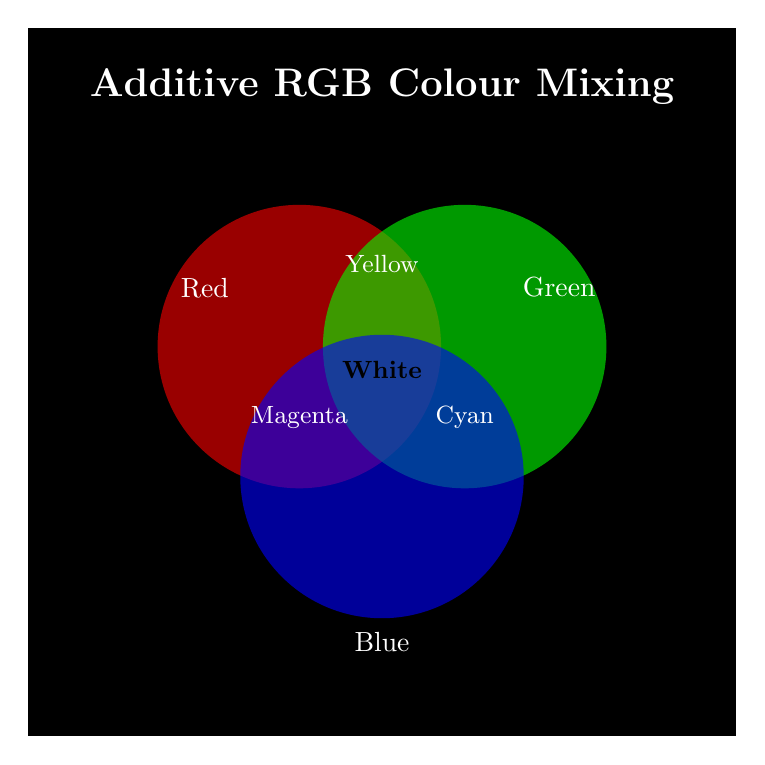
\begin{tikzpicture}[scale=1.5]
  % Background
  \fill[black] (-3,-3) rectangle (3,3);
  
  % Title
  \node[white, font=\Large\bfseries] at (0, 2.5) 
    {Additive RGB Colour Mixing};
  
  % Red circle
  \fill[red, opacity=0.6] (-0.7, 0.3) circle (1.2);
  
  % Green circle
  \fill[green, opacity=0.6] (0.7, 0.3) circle (1.2);
  
  % Blue circle
  \fill[blue, opacity=0.6] (0, -0.8) circle (1.2);
  
  % Labels
  \node[white] at (-1.5, 0.8) {Red};
  \node[white] at (1.5, 0.8) {Green};
  \node[white] at (0, -2.2) {Blue};
  
  % Secondary colours (approximate positions)
  \node[white, font=\small] at (-0.7, -0.3) {Magenta};
  \node[white, font=\small] at (0.7, -0.3) {Cyan};
  \node[white, font=\small] at (0, 1.0) {Yellow};
  
  % Center white
  \node[black, font=\small\bfseries] at (0, 0.1) {White};
\end{tikzpicture}

\end{document}